\section{Diagonalized Mixed-Hybrid Method}
\def\mr{\mathring}
Model of flow described in section \ref{sec:darcy_flow} is solved by
the mixed-hybrid formulation (MH) of the finite element method.
As in the previous chapter, let
$\tau$ be the time step and $\mathcal T_d$ a regular simplicial partition of $\Omega_d$, $d=1,2,3$.
Denote by $\vc W_d(T_d)\subset \vc H(div,T_d)$
 the space of Raviart-Thomas functions of order zero ($RT_0$) on an element $T_d\in 
\mathcal T_d$.
We introduce the following spaces:
\[
    \vc W =  \vc W_1 \times \vc W_2 \times \vc W_3,\quad
    \vc W_d = \prod_{T_d\in \mathcal T_d} \vc W_d(T_d),
\]
\begin{equation}
Q=Q_{1}\times Q_{2}\times Q_{3},
\quad
Q_{d}=L^{2}\left(  \Omega_{d}\right).
\end{equation}
For every $T_d\in \mathcal T_d$ we define the auxiliary space of values on interior sides of $T_d$:
\begin{equation}
    \mr Q(T_d)=\left\{  \mr q\in 
    L^{2}(\partial T_d \setminus  \partial\Omega_d^D):
    \mr q =\vc w\cdot \vc n|_{\partial T_d},
    \vc w\in\vc W_d%
    \right\}.
\end{equation}
Further we introduce the space of functions defined on interior sides that do not coincide with elements of the lower dimension:
\begin{equation}
    \mr Q_d=\Big\{
        \mr q\in\prod_{T \in \mathcal T_d} \mr Q(T);
        \ \mr q|_{\partial T}=\mr q|_{\partial \tilde T}%
        \quad\text{on the side }F=\partial T\cap\partial \tilde T
        \quad\text{ if }F\cap\Omega_{d-1}=\emptyset
    \Big\}.
\end{equation}
Finally we set $\mr Q = \mr Q_1 \times \mr Q_2 \times \mr Q_3$.

The \emph{mixed-hybrid method} for the unsteady Darcy flow reads as follows.
We are looking for a trio $(\mathbf{u},h,\mr h)  
\in \vc W\times Q\times\mr Q$ which satisfies the saddle-point problem:
\begin{align}
    a(\vc u,\vc v)  +b(\vc v, p) + \mr b(\vc v, \mr p)
        &=\langle g,\vc v \rangle, \qquad\forall \vc v\in \vc W,
        \label{eq:hybrid-frac-1}\\
    b(\vc u, q ) + \mr b( \vc u, \mr q) - c(p, \mr p, q, \mr q)
        &= \langle f, (q,\mr q) \rangle,
        \qquad\forall q\in Q,\ \mr q\in \mr Q, 
        \label{eq:hybrid-frac-2}
\end{align}
where
\begin{align}
    \label{eq:weak_term_a}
    a(\vc u, \vc v) &= \sum_{d=1}^{3}\sum_{T\in \mathcal T_d}
    \int_{T} \frac{1}{\delta_{d}}\tn K_{d}^{-1} 
    \vc u_d\cdot \vc v_d\,dx,
    \\
    \label{eq:weak_term_b}
    b(\vc u, q)  &= -\sum_{d=1}^{3}\sum_{T\in \mathcal T_d}
    \int_{T} q_d\,\div \vc u_d\,dx,
    \\
    \label{eq:weak_term_bf}
    \mr b(\vc u, \mr q)   &= \sum_{d=1}^{3}\sum_{T\in \mathcal T_d}
    \int_{\partial T\setminus\partial\Omega_{d}}
        \mr q|_{\partial T} ( \vc u_d\cdot\vc n)\,ds,
    \\
    \label{eq:weak_term c}
    c(h, \mr h, q, \mr q) &= c_f(h, \mr h, q, \mr q) 
    + c_t(h, \mr h, q, \mr q) + c_R(\mr h, \mr q)
    \\
    c_f(h, \mr h, q, \mr q)&=\sum_{d=2,3}\sum_{T\in \mathcal T_d}
        \int_{\partial T \cap\Omega_{d-1}} \sigma_{d} 
        (p_{d-1} - \mr p_d)(q_{d-1} - \mr q_d)\,ds
    \\
    c_t(h, \mr h, q, \mr q)&= \sum_{d=1}^{3}\sum_{T\in \mathcal T_d}
        \int_{T} \frac{\delta_d S_d}{\tau} h_d q_d\,dx,
    \\    
    c_R(\mr h, \mr q)&= \sum_{d=1}^{3}\sum_{T\in \mathcal T_d}
    \int_{\partial T\cap\Gamma_{d}^{TF}}
        \sigma_d^R\, h_d \mr q_d \,ds,
    \\
    \langle g, \vc v \rangle  & =
    -\sum_{d=1}^{3}\sum_{T\in\mathcal T_d}
    \int_{\partial T\cap\partial\Omega_N} 
        p_d^D\, (\vc v \cdot \vc n)  \,ds,
    \\
    \langle f, q \rangle  &=
    -\sum_{d=1}^{3}\int_{\Omega_d} \delta_{d}\,f_d\,q_{d}\,dx,
    \\
        &\phantom{=}-
    \sum_{d=1}^{3}\sum_{T\in\mathcal T_d}
    \int_{\partial T\cap\Gamma_d^{TF}} 
        q_d^N \mr q_d + \sigma_d^R\, h_d^R \mr q_d\,ds
    \\
        &\phantom{=}-c_t(\tilde h, \mr{\tilde{h}}, q, \mr q).
    \label{eq:weak_term_f}%    
\end{align}
All quantities are meant in time $t$, only $\tilde h$ is the pressure head in time $t-\tau$.

The advantage of the mixed-hybrid method is that the set of equations $\eqref{eq:hybrid-frac-1} - 
\eqref{eq:hybrid-frac-2}$ can be reduced by eliminating the unknowns $\vc u$ and $q$
to a sparse positive definite system for $\mr q$.
This equation can then be efficiently solved using a~preconditioned conjugate gradient method.
Unfortunately, it appears that the resulting system does not satisfy the discrete maximum principle
 which in particular for short time steps $\tau$ can lead to unphysical oscillations.
One possible solution is the diagonalization of the method (lumped mixed-hybrid method, LMH)
 proposed in \cite{younes_2006}.
This method was implemented in Flow123d as well.
It consists in replacing the form $c_t$ by
\[
    c_t(h, \mr h, q, \mr q)= \sum_{d=1}^{3}\sum_{T\in \mathcal T_d}
        \sum_{i=1}^{d+1} \alpha_{T,i} \abs{T} \frac{\delta_d S_d}{\tau} 
        \left(\mr h|_{S_{T,i}}\,  \mr q|_{S_{T,i}}\right),
\]
and the source term $\sum_{d=1}^{3}\int_{\Omega_d} \delta_{d}\,f_d\,q_{d}\,dx$ by
\[
    \sum_{d=1}^{3}\sum_{T\in \mathcal T_d}
        \sum_{i=1}^{d+1} \alpha_{T,i} \abs{T} \delta_d f_d\,
        \mr q|_{S_{T,i}},
\]
where $\abs{T}$ is the size of an element $T$, $S_{T,i}$ is the $i$-th side of $T$, and 
$\mr h|_{S_{T,i}}$ is the degree of freedom on the side $S_{T,i}$. 
Weights $\alpha_{T,i}$ can be chosen to be $1/(d+1)$. 
After solving the set of equations it is necessary to modify the velocity field $\vc u$
 by adding the time term.
This modified system already satisfies the discrete maximum principle
 and does not produce oscillations.
Figure \ref{fig:LMH} shows a comparison of the results
 using conventional MH scheme and LMH scheme.
At the MH scheme one can observe oscillations in the wavefront
 where the minimum value is significantly less than zero.

\begin{figure}
    \begin{center}
       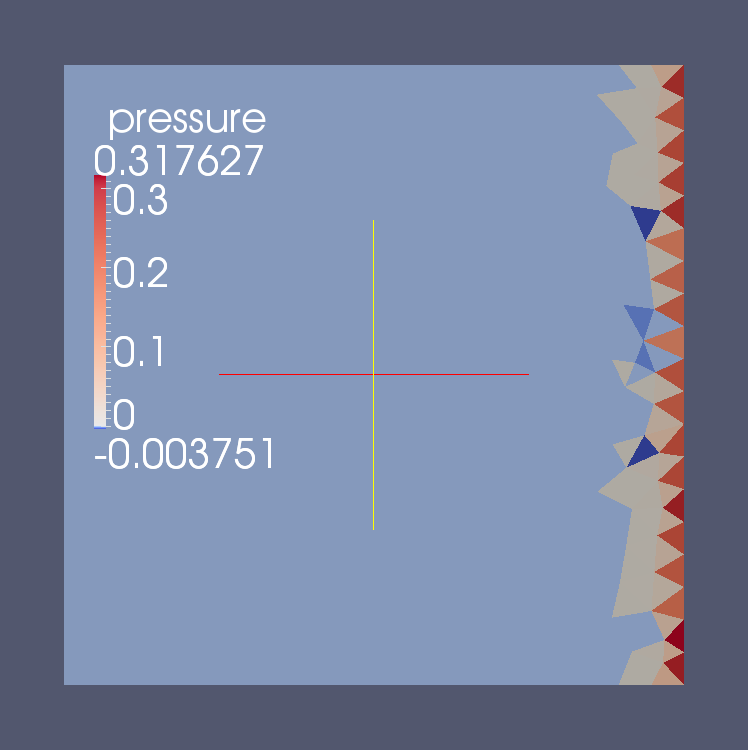
\includegraphics[width=0.4\textwidth]{figures/MH.png}
       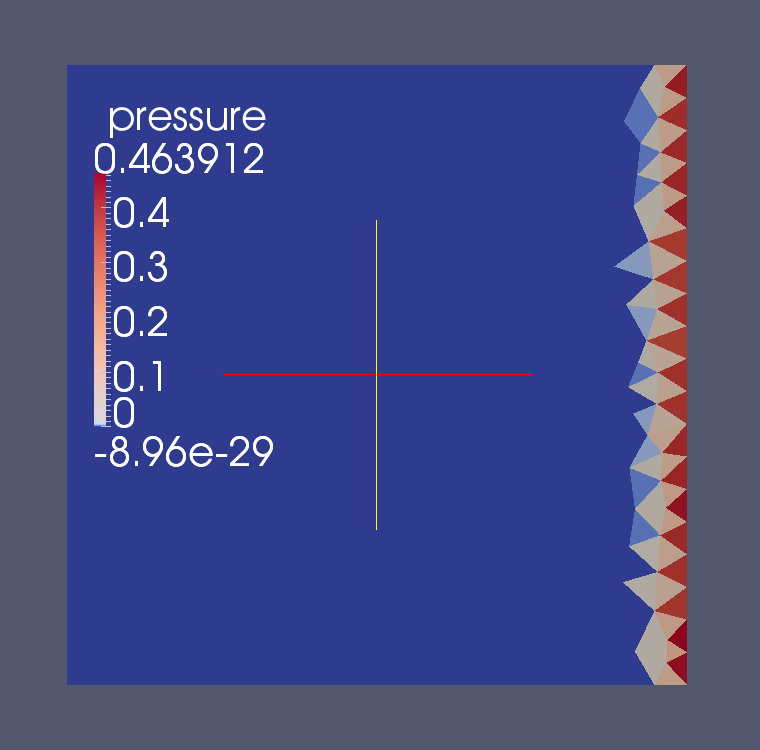
\includegraphics[width=0.405\textwidth]{figures/LMH.png}        
    \end{center}
    \caption{Comparison of MH (left) and LMH scheme (right), $\tau=10^{-4}$.}
    \label{fig:LMH}
\end{figure}

